% Copyright 2020  Ed Bueler

\documentclass[10pt,hyperref,dvipsnames]{beamer}

\mode<presentation>{
  \usetheme{Madrid}
  \usecolortheme{beaver}
  \setbeamercovered{transparent}  
  \setbeamerfont{frametitle}{size=\large}
}

\setbeamercolor*{block title}{bg=red!10}
\setbeamercolor*{block body}{bg=red!5}

\usepackage[english]{babel}
\usepackage[latin1]{inputenc}
\usepackage{times}
\usepackage[T1]{fontenc}
% Or whatever. Note that the encoding and the font should match. If T1
% does not look nice, try deleting the line with the fontenc.

\usepackage{empheq}
\usepackage{xspace}
\usepackage{verbatim,fancyvrb}

\usepackage{tikz}
\usetikzlibrary{shapes,arrows.meta,decorations.markings,decorations.pathreplacing,fadings,positioning}

\usepackage{hyperref}

% If you wish to uncover everything in a step-wise fashion, uncomment
% the following command: 
%\beamerdefaultoverlayspecification{<+->}

\newcommand{\ba}{\mathbf{a}}
\newcommand{\bb}{\mathbf{b}}
\newcommand{\bc}{\mathbf{c}}
\newcommand{\bbf}{\mathbf{f}}
\newcommand{\bg}{\mathbf{g}}
\newcommand{\bq}{\mathbf{q}}
\newcommand{\br}{\mathbf{r}}
\newcommand{\bx}{\mathbf{x}}
\newcommand{\by}{\mathbf{y}}
\newcommand{\bv}{\mathbf{v}}
\newcommand{\bu}{\mathbf{u}}
\newcommand{\bw}{\mathbf{w}}

\newcommand{\bF}{\mathbf{F}}
\newcommand{\bG}{\mathbf{G}}
\newcommand{\bQ}{\mathbf{Q}}

\newcommand{\grad}{\nabla}
\newcommand{\Div}{\nabla\cdot}
\newcommand{\minmod}{\operatorname{minmod}}

\newcommand{\CC}{\mathbb{C}}
\newcommand{\RR}{\mathbb{R}}

\newcommand{\ddt}[1]{\ensuremath{\frac{\partial #1}{\partial t}}}
\newcommand{\ddx}[1]{\ensuremath{\frac{\partial #1}{\partial x}}}
\newcommand{\Matlab}{\textsc{Matlab}\xspace}
\newcommand{\Octave}{\textsc{Octave}\xspace}
\newcommand{\eps}{\epsilon}

\newcommand{\ip}[2]{\left<#1,#2\right>}

\newcommand{\xiphalf}{{x_{i+\frac{1}{2}}}}
\newcommand{\ximhalf}{{x_{i-\frac{1}{2}}}}
\newcommand{\Fiphalf}{{F_{i+\frac{1}{2}}}}
\newcommand{\Fimhalf}{{F_{i-\frac{1}{2}}}}
\newcommand{\Fiphalfn}{{F^n_{i+\frac{1}{2}}}}
\newcommand{\Fimhalfn}{{F^n_{i-\frac{1}{2}}}}

\newcommand{\trefcolumn}[1]{\begin{bmatrix} \phantom{x} \\ #1 \\ \phantom{x} \end{bmatrix}}
\newcommand{\trefmatrixtwo}[2]{\left[\begin{array}{c|c|c} & & \\ #1 & \dots & #2 \\ & & \end{array}\right]}
\newcommand{\trefmatrixthree}[3]{\left[\begin{array}{c|c|c|c} & & & \\ #1 & #2 & \dots & #3 \\ & & & \end{array}\right]}
\newcommand{\trefmatrixgroups}[4]{\left[\begin{array}{c|c|c|c|c|c} & & & & & \\ #1 & \dots & #2 & #3 & \dots & #4 \\ & & & & & \end{array}\right]}

\newcommand{\blocktwo}[4]{\left[\begin{array}{c|c} #1 & #2 \\ \hline #3 & #4 \end{array}\right]}

\newcommand{\bqed}{{\color{blue}\qed}}
\newcommand{\ds}{\displaystyle}

\newcommand\mynum[1]{{\renewcommand{\insertenumlabel}{#1}%
      \usebeamertemplate{enumerate item} \,}}


\title[Finite volume methods]{Finite volume methods for \\ advection equations and hyperbolic systems}

%\subtitle{part I: xx}

\author{Ed Bueler}

\institute[UAF]{University of Alaska Fairbanks}

\date{June 2020}

% this nonsense needed to start section counter at 0; see
% https://tex.stackexchange.com/questions/170222/change-the-numbering-in-beamers-table-of-content
\makeatletter
\patchcmd{\beamer@sectionintoc}
  {\ifnum\beamer@tempcount>0}
  {\ifnum\beamer@tempcount>-1}
  {}
  {}
\beamer@tocsectionnumber=-1
\makeatother


\begin{document}
\beamertemplatenavigationsymbolsempty

\begin{frame}
  \maketitle
\end{frame}

\begin{frame}
  \frametitle{Outline}
  \tableofcontents[hideallsubsections]
\end{frame}


\section{overview}

\begin{frame}[fragile]
\frametitle{overview}

\begin{itemize}
\item numerical solutions of systems of first-order, time-dependent PDEs
    \begin{itemize}
    \item[$\circ$] finite volume (FV) methods
    \item[$\circ$] a genuine introduction
    \end{itemize}
\item we will solve these hyperbolic equations:

\bigskip
\begin{center}
\begin{tikzpicture}[scale=0.9,
                    >={Latex[length=2mm]},
  eqn/.style={
     rectangle,draw,fill=white,align=center,line width=0.6pt,minimum width=15mm}]

%center
\draw[line width=1pt] (0,0)     node[eqn] (scalaradvect)  {\mynum{1} scalar advection \\ {\Large \strut} $q_t + a q_x=0$};
\draw[line width=1pt] (3,-1.7)     node[eqn] (scalartwod)  {\mynum{5} scalar advection in 2D \\ {\Large \strut} $q_t + (u q)_x + (v q)_y=0$};
\draw[line width=1pt] (-2,-1.7)    node[eqn] (linearsystem)  {\mynum{2} linear systems \\ {\Large \strut} $\bq_t + A\, \bq_x=0$};
\draw[line width=1pt] (-2,-3.55)    node[eqn] (generalsystem)  {\mynum{4} conservation-law systems \\ {\Large \strut} $\bq_t + \bF(t,x,\bq)_x=\bg(t,x,\bq)$};

\path[-Latex]
   ([xshift=-2em]scalaradvect.south) edge node {} (linearsystem)
   ([xshift=2em]scalaradvect.south) edge node {} (scalartwod)
   (linearsystem.south) edge node {} (generalsystem);
\end{tikzpicture}

\bigskip
    \begin{itemize}
    \item[$\circ$] ``hyperbolic'' (defined in part \mynum{2}) means finite speed of influence
    \item[$\circ$] arrows show generalizations
    \end{itemize}
\end{center}
\end{itemize}
\end{frame}


\begin{frame}{references}
\begin{itemize}
\item {\large \alert{R.~J.~LeVeque, \emph{Finite Volume Methods for Hyperbolic Problems}, Cambridge University Press, 2002}}

\bigskip
\item K.~W.~Morton and D.~F.~Mayers, \emph{Numerical Solutions of Partial Differential Equations: An Introduction}, Cambridge University Press, 2nd ed., 2005
\item W.~Hundsdorfer and J.~G.~Verwer, \emph{Numerical Solution of Time-Dependent Advection-Diffusion-Reaction Equations}, Springer, 2003
\item E.~Bueler, \emph{PETSc for Partial Differential Equations}, SIAM Press, 2020?
\end{itemize}
\end{frame}


\begin{frame}{visual example 1: numerical solution}

\begin{itemize}
\item before getting to numerical solutions, some show-and-tell \dots two movies
\item consider advection equation for scalar density $q(t,x)$:
    $$q_t + a \, q_x = 0$$
with speed $a=1$, initial condition $q(0,x)$ known, and periodic boundary conditions on $0\le x \le 1$
\item movie of numerical solution for $0\le t \le 1$
    \begin{itemize}
    \item[$\circ$] initial shape is transported from initial position back to same position
    \end{itemize}
\end{itemize}

\vspace{10mm}
\begin{center}
\alert{SHOW MOVIE}
\end{center}
\vspace{10mm}

% cd p4pdes-next/riemann/
% make riemann
% ./riemann -problem advection -da_grid_x 200 -limiter minmod -ts_monitor_solution binary:q.dat -ts_monitor binary:t.dat
% make petscPyScripts
% mkdir advection
% ./plotTS.py -mx 200 -ylabel "q" -ax 0.0 -bx 1.0 -cellcentered t.dat q.dat -oroot advection/bar
% cd advection
% eog bar*.png
\end{frame}


\begin{frame}{visual example 1: numerical \emph{and exact} solutions}

\begin{itemize}
\item was it clear what the movie showed?
\item compare when we have the exact solution:
\end{itemize}

\bigskip
\hfill \mbox{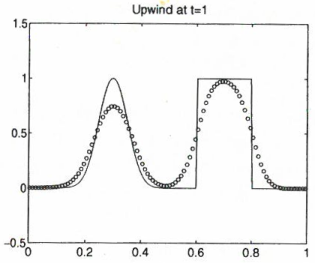
\includegraphics[width=0.48\textwidth]{figs/leveque6p1upwind} \, 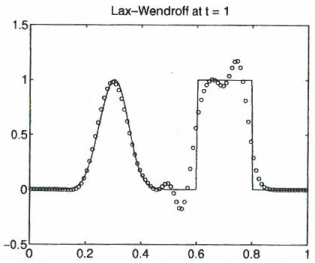
\includegraphics[width=0.48\textwidth]{figs/leveque6p1lw}}
\end{frame}


\begin{frame}{visual example 2: merely a numerical solution}

\begin{itemize}
\item shallow water water equations:

\vspace{-11.5mm}
\begin{align*}
\hspace{60mm} h_t + (hu)_x &= 0 \\
(hu)_t + \left(h u^2 + \frac{g}{2} h^2\right)_x &= 0
\end{align*}
\item suppose initial condition is a ``hump'' on $x\in[-5,5]$
    \begin{itemize}
    \item[$\circ$] $h(0,x)=a e^{-bx^2}$, $u(0,x)=0$, thus
    \item[$\circ$] vertical displacement in the center of the domain
    \item[$\circ$] simplest model for a tsunami from block fault in middle of ocean?
    \end{itemize}
\item movie of numerical solution for $0 \le t \le 18$

\vspace{10mm}
\begin{center}
\alert{SHOW MOVIE}
\end{center}

\vspace{10mm}

% ./riemann -problem swater -initial hump -da_grid_x 1000 -limiter minmod -ts_monitor binary:t.dat -ts_monitor_solution binary:q.dat
% mkdir swater
% ./plotTS.py -mx 1000 -ylabel "h (height)" -ax -5.0 -bx 5.0 -dof 2 -c 0 -cellcentered t.dat q.dat -oroot swater/bar
% cd swater
% eog bar*.png
\end{itemize}
\end{frame}


\begin{frame}{roles for exact solutions}

\begin{itemize}
\item exact solutions are needed for \emph{verifying} simulations
    \begin{itemize}
    \item[$\circ$] i.e.~measure norm of difference between exact and numerical solutions
    \item[$\circ$] they are precise tools for ``mathematical engineering'' of numerical solvers
    \end{itemize}
\item also: numerical solvers for hyperbolic systems use a ``Riemann solver'' 
    \begin{itemize}
    \item[$\circ$] essentially an exact solution for a discontinuous initial condition
    \item[$\circ$] explaining this is a main goal of my talk
    \end{itemize}
\item generally, exact solutions are rare but valuable
\end{itemize}
\end{frame}


\begin{frame}{high performance and parallel}

\begin{itemize}
\item I am interested in high performance and parallel solutions of PDEs
    \begin{itemize}
    \item[$\circ$] so I am mostly not using \Matlab or Python/scipy
    \end{itemize}
\item movies in these slides were generated by C programs which call PETSc, the Portable Extensible Toolkit for Scientific computing:

    \begin{center}
    \href{https://www.mcs.anl.gov/petsc/}{\texttt{www.mcs.anl.gov/petsc/}}
    \end{center}

    \begin{itemize}
    \item[$\circ$] it is a mathematical library for high-performance computing
    \item[$\circ$] PETSc is brought to you by the same people who brought you MPI
    \end{itemize}
\item speed and parallelizability are nice for one spatial dimension, but \emph{critical} for 2D and 3D
\end{itemize}

\vspace{10mm}
\begin{center}
\alert{SHOW COMPUTATION OF SHALLOW WATER MOVIE}
\end{center}

% ./riemann -problem swater -initial hump -da_grid_x 1000 -limiter minmod -ts_monitor binary:t.dat -ts_monitor_solution binary:q.dat
\end{frame}


\begin{frame}{please ask questions}

\begin{itemize}
\item the rest of the talk is about the math not the movies
    \begin{itemize}
    \item[$\circ$] but lots of figures to explain concepts
    \end{itemize}
\item \alert{PLEASE} ask lots of questions, about any topic at all
    \begin{itemize}
    \item[$\circ$] slowing me down is a \emph{good} thing!
    \end{itemize}
\end{itemize}
\end{frame}


\AtBeginSection[]
{
  \begin{frame}<beamer>
    \frametitle{Outline}
    \tableofcontents[currentsection,hideallsubsections]
  \end{frame}
}

\section{scalar advection equation}

\begin{frame}{one-way advection}

\begin{itemize}
\item the \emph{scalar advection equation (PDE)} for $q(t,x) \in \RR$:
    $$q_t + a q_x=0$$

    \begin{itemize}
    \item[$\circ$] $a\in\RR$ constant on this slide
    \end{itemize}
\item if we have initial condition $q(t,0)=f(x)$, with $f(x)$ smooth, then the solution is
    $$q(t,x) = f(x-at)$$
\item \emph{because}, by the chain rule
    $$q_t(t,x) = f'(x-at) (-a) \quad \text{ and } \quad q_x(t,x) = f'(x-at)$$
so $q_t + a q_x = -a f'(x-at) + a f'(x-at) = 0$
\item the solution $q(t,x)=f(x-at)$ is a movie of the graph of $f(x)$ translating to the right by $at$ in time $t$
    \begin{itemize}
    \item[$\circ$] even if $a$ and/or $t$ are negative
    \item[$\circ$] note $a$ is the speed of the motion
    \end{itemize}
\end{itemize}
\end{frame}


\begin{frame}{solution by characteristics}

\begin{itemize}
\item but what about the scalar PDE with variable speed $a(t,x)$?:
    $$q_t + a(t,x) q_x=0, \qquad q(0,x) = f(x)$$
\item we need the idea of a \emph{characteristic curve} (ODE):
    $$\ds \frac{d\xi}{ds} = a(s,\xi(s)) \hspace{50mm}$$

\vspace{-10mm}

\hfill 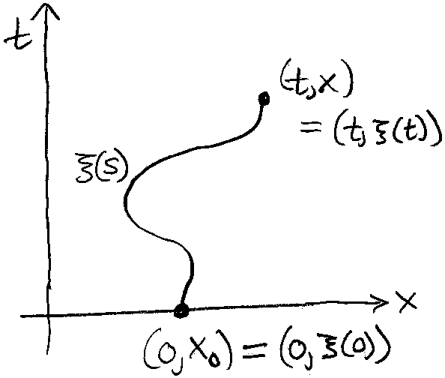
\includegraphics[width=0.32\textwidth]{figs/characteristicsketch}

\vspace{-20mm}
\item for a solution $q(t,x)$, we calculate $\left[\xi'=\tfrac{d\xi}{ds}\right]$
\begin{align*}
\Big(q(s,\xi(s))\Big)' &= q_t(s,\xi(s)) + q_x(s,\xi(s)) \xi'(s) \hspace{40mm} \\
                          &= q_t(s,\xi(s)) + q_x(s,\xi(s)) a(s,\xi(s)) \\
                          &= 0,
\end{align*}
\item thus $q(t,\xi(t)) = q(0,\xi(0))$
\item \emph{solution by characteristics}: $q(t,x)$ has the same value as $f(x_0)$ if $\xi(s)$ is a characteristic curve that ends at $(t,x)$ and starts at $(0,x_0)$
\end{itemize}
\end{frame}


\begin{frame}{solution by characteristics 2}

\begin{itemize}
\item the method can be extended to the possibly-nonlinear equation
     $$q_t + a(t,x) q_x = g(t,x,q), \qquad q(0,x) = f(x)$$

    \begin{itemize}
    \item[$\circ$] $a$ is the speed of the characteristic curve
    \item[$\circ$] $g$ is the \emph{source term}
    \item[$\circ$] solution $q$ changes at rate $g$ along the characteristic
    \item[$\circ$] if $g=0$ then $q$ is constant along the characteristic
    \end{itemize}
\item now a pair of ODEs to solve:
\begin{align*}
\xi'(s) &= a(s,\xi(s)) \\
\omega'(s) &= g(s,\xi(s),\omega(s))
\end{align*}
\item \emph{solution by characteristics}:
    \begin{itemize}
    \item[i)] from 1st ODE, find characteristic $\xi(s)$ through $(0,x_0)$ and $(t,x)$
    \item[ii)] solve 2nd ODE with initial condition $\omega(0)=f(x_0)$
    \item[iii)] then $q(t,x) = \omega(t)$
    \end{itemize}
\item \alert{main idea} about advection PDEs:

\begin{center}
information travels along the characteristics
\end{center}
\end{itemize}
\end{frame}


\begin{frame}{upwind scheme for one-way advection}

\begin{itemize}
\item apply \emph{upwind} scheme to $q_t + aq_x=0$ in case $a>0$:
    $$\frac{Q_i^{n+1} - Q_i^n}{\Delta t} + a \frac{Q_i^n - Q_{i-1}^n}{\Delta x} = 0$$
\item equivalently, solve for the new value at $t_{n+1}$:
\begin{align*}
Q_i^{n+1} &= \frac{a\Delta t}{\Delta x} Q_{i-1}^n + \left(1 - \frac{a\Delta t}{\Delta x}\right) Q_i^n = \ell(x_i-a\Delta t)
\end{align*}
where $\ell(x)$ linearly interpolates

\noindent between $(x_{i-1},Q_{i-1}^n)$ and $(x_i,Q_i^n)$

\vspace{-9mm}
\hfill 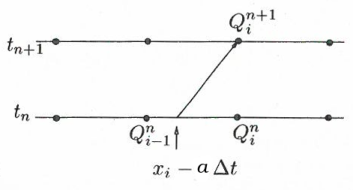
\includegraphics[width=0.45\textwidth]{figs/leveque4p4a}

\vspace{-7mm}
\item interpolate $\ell$ where the characteristic

\noindent through $(x_i,Q_i^{n+1})$ hits the $t_n$ line

\item except we must require \emph{interpolation} instead of extrapolation: $\ds \frac{|a|\Delta t}{\Delta x} \le 1$
\end{itemize}
\end{frame}


\begin{frame}{upwind and Lax-Wendroff schemes}

\begin{itemize}
\item while upwind uses linear interpolation using two points, \dots
\item the \emph{Lax-Wendroff} scheme uses quadratic interpolation with three points
\item for formulas, let $\nu = a\Delta t/\Delta x$; then
\begin{align*}
Q_i^{n+1} &= \nu Q_{i-1}^n + \left(1 - \nu\right) Q_i^n \\
Q_i^{n+1} &= \tfrac{1}{2} \nu (1+\nu) Q_{i-1}^n + \left(1 - \nu^2\right) Q_i^n + \tfrac{1}{2} \nu (1-\nu) Q_{i+1}^n
\end{align*}

\begin{center}
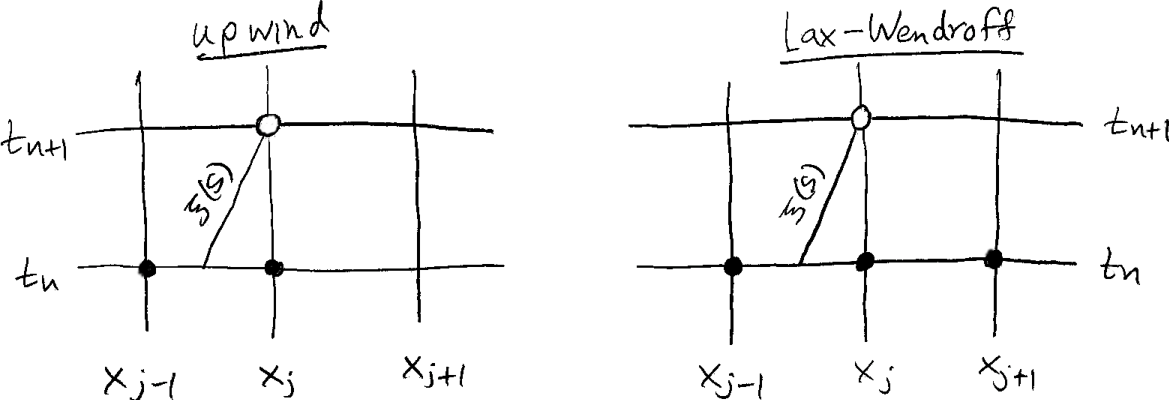
\includegraphics[width=0.95\textwidth]{figs/stencilssketch}
\end{center}
\end{itemize}
\end{frame}


\begin{frame}{stability}

\begin{itemize}
\item \emph{BUT} we still need CFL so that these upwind and Lax-Wendroff formulas are \emph{interpolations} not \emph{extrapolations}:
    $$|\nu| = \frac{|a|\Delta t}{\Delta x} \le 1 \qquad \iff \qquad \Delta t \le \frac{\Delta x}{|a|}$$

    \begin{itemize}
    \item[$\circ$] the errors from extrapolation are known to propagate forward, time step by time step, as exponential growth, i.e.~\emph{unstably}
    \end{itemize}
\item essentially the same can be said for any finite difference, finite volume, or finite element scheme for hyperbolic PDEs:

\begin{center}
a CFL condition is \emph{necessary} for stability (and thus for convergence)
\end{center}

\item \alert{main idea of CFL:} the characteristic(s) through the new location $(t_{n+1},x_i)$ must pass through the numerical ``domain of dependence'' of the scheme at the old time $t_n$
\end{itemize}
\end{frame}


\begin{frame}{results}

\begin{itemize}
\item suppose same problem as in earlier movie:

$q_t+a q_x=0$, $a=1$, $0\le x\le 1$, and periodic boundary conditions

\medskip
\hfill 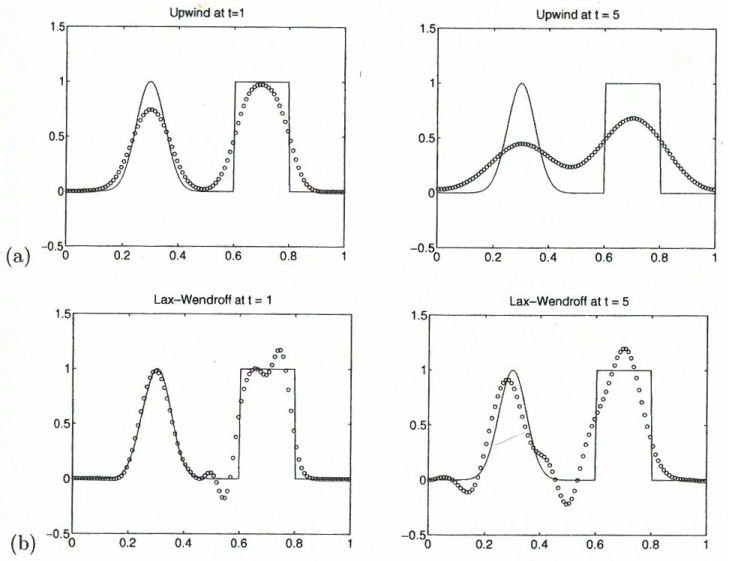
\includegraphics[width=0.72\textwidth]{figs/leveque6p1}

\vspace{-25mm}

\alert{\emph{issues:}

{\footnotesize oversmoothing}

{\footnotesize oscillation}

{\footnotesize loss of original bounds}}
\end{itemize}
\end{frame}


\begin{frame}{how to do better? \dots the historical picture}

\begin{itemize}
\item the results above suffer from three diseases:
    \begin{itemize}
    \item[$\circ$] \alert{oversmoothing} (upwind)
    \item[$\circ$] \alert{oscillation} (Lax-Wendroff)
    \item[$\circ$] \alert{loss of original solution bounds} (Lax-Wendroff)
    \end{itemize}

\vspace{-15mm}

\hfill 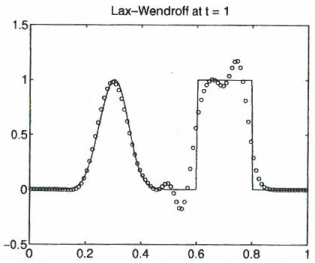
\includegraphics[width=0.3\textwidth]{figs/leveque6p1lw}

\bigskip
\item upwind and Lax-Wendroff were clear to everyone by $\sim$1960
    \begin{itemize}
    \item[$\circ$] upwind and Lax-Wendroff were regarded as \emph{finite difference} methods
    \end{itemize}
\item in 1970--90s these diseases were mostly fixed \dots how?:
    \begin{itemize}
    \item[$\circ$] ``finite volume'' thinking
    \item[$\circ$] ``Riemann solver'' interpretation of the upwind method
    \item[$\circ$] ``slope-limiting'' or ``flux-limiting'' to avoid oscillations
    \item[$\circ$] this talk: make sense of these new buzzwords!
    \end{itemize}
\end{itemize}
\end{frame}


\begin{frame}{the finite volume (FV) idea}

\begin{itemize}
\item assume the problem is in flux-conservation form
    $$q_t + f(q)_x = 0$$

    \begin{itemize}
    \item[$\circ$] $f(q) = aq$ in scalar advection $q_t + a q_x = 0$
    \end{itemize}
\item put a grid on $x$: suppose $x_i$ is center of a \emph{cell}, and integrate over the cell:
\begin{gather*}
\int_\ximhalf^\xiphalf q_t + f(q)_x \,dx = 0 \hspace{20mm}  \\
\frac{d}{dt} \int_\ximhalf^\xiphalf q(t,x) \,dx + f\left(q(t,\xiphalf)\right) - f\left(q(t,\ximhalf)\right) = 0
\end{gather*}

\vspace{-4mm}
\hfill 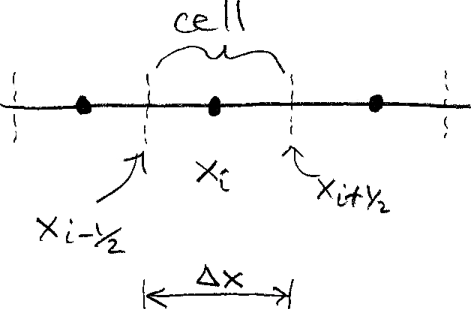
\includegraphics[width=0.27\textwidth]{figs/fvsketch}

\vspace{-20mm}
\item interpret: $\ds Q_i(t) \approx \frac{1}{\Delta x} \int_\ximhalf^\xiphalf q(t,x)\,dx$
    \begin{itemize}
    \item[$\circ$] versus in a finite difference scheme: $Q_i^n \approx q(t_n,x_i)$
    \end{itemize}
\item also, $\Fiphalf(t) \approx f\left(q(t,\xiphalf)\right)$ is flux at \emph{cell face}
\end{itemize}
\end{frame}


\begin{frame}{the FV idea 2}

\begin{itemize}
\item suppose we put a grid on $t$ and use forward Euler in time
\item now we have this sequence of equations:
\small
\begin{gather*}
q_t + f(q)_x = 0 \hspace{50mm} \\
\frac{d}{dt} \int_\ximhalf^\xiphalf q(t,x) \,dx + f\left(q(t,\xiphalf)\right) - f\left(q(t,\ximhalf)\right) = 0 \hspace{50mm} \\
\frac{dQ_i}{dt} + \Fiphalf - \Fimhalf = 0 \hspace{50mm} \\
\Delta x \left(\frac{Q_i^{n+1} - Q_i^n}{\Delta t}\right) + \Fiphalfn - \Fimhalfn = 0 \hspace{50mm} \\
\alert{\frac{Q_i^{n+1} - Q_i^n}{\Delta t} + \frac{\Fiphalfn - \Fimhalfn}{\Delta x} = 0} \hspace{50mm}
\end{gather*}

\vspace{-15mm}

\hfill 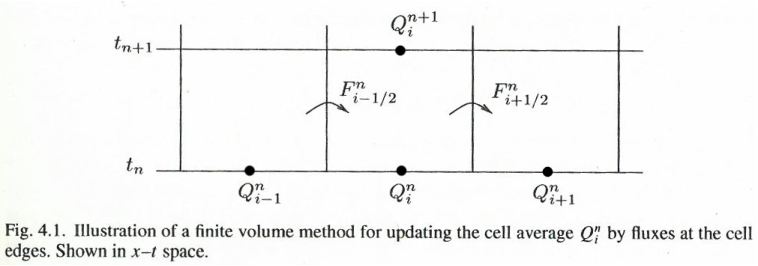
\includegraphics[width=0.45\textwidth]{figs/leveque4p1}

\normalsize
\medskip
\item the \alert{last equation} is a computable numerical scheme \emph{if} we have a scheme for approximating the face fluxes $\Fiphalfn$
\item note we distinguish $q(t_n,x_i)$ and $Q_i^n$ \quad \dots you should too!
\end{itemize}
\end{frame}


\begin{frame}{method-of-lines (MOL) thinking}

\begin{itemize}
\item \emph{but} we should not commit to forward Euler so soon!
\item suppose again: $\ds Q_i(t) \approx \frac{1}{\Delta x} \int_\ximhalf^\xiphalf q(t,x)\,dx$ and $\Fiphalf(t) \approx f\left(q(t,\xiphalf)\right)$
\item then integrating $q_t + f(q)_x = 0$

over the cell gives
    $$\frac{dQ_i}{dt} + \frac{\Fiphalf-\Fiphalf}{\Delta x} = 0, \hspace{60mm}$$

the basic FV scheme

\vspace{-24mm}
\hfill 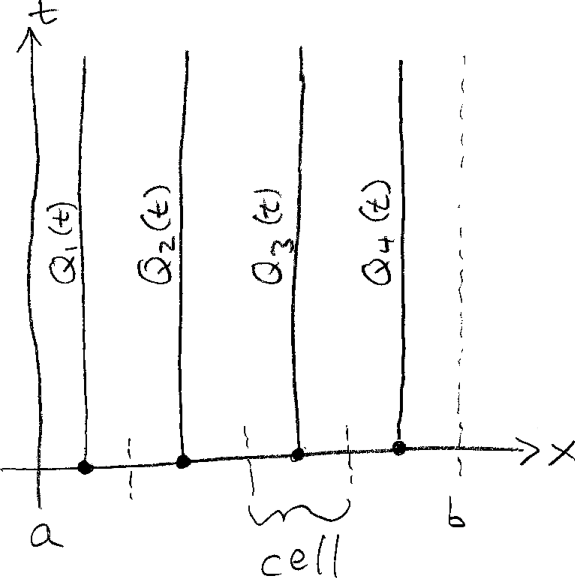
\includegraphics[width=0.42\textwidth]{figs/molsketch}

\vspace{-21mm}
\item this is a system of ODEs in time
    $$\frac{d\bQ}{dt} = \bG(t,\bQ), \quad \bQ(t) = \begin{bmatrix} Q_1(t) \\ \vdots \\ Q_J(t) \end{bmatrix}   \hspace{60mm}$$

\item why? because good black-box ODE solvers are already available
    \begin{itemize}
    \item[$\circ$] \texttt{ode23}, etc. \qquad \dots it is not 1970 anymore, people!
    \end{itemize}
\end{itemize}
\end{frame}


\begin{frame}{upwind again, as ``donor cell'' method}

\begin{itemize}
\item the classic upwind method for $q_t + a q_x = 0$, when regarded in FV terms, amounts to three things:
    \begin{itemize}
    \item[i)] integrate over the spatial cell (FV MOL):
        $$\frac{dQ_i}{dt} + \frac{\Fiphalf-\Fiphalf}{\Delta x} = 0 \hspace{50mm}$$
    \item[ii)] compute flux $F(q)=aq$ from the upwind \emph{donor cell}:
        $$\Fiphalf = \begin{cases} a Q_{i}, & a \ge 0, \\
                                   a Q_{i+1}, & a < 0 \end{cases} \hspace{50mm}$$
    \item[iii)] forward Euler for time stepping:
        $$\frac{Q_i^{n+1} - Q_i^n}{\Delta t} + a \frac{\begin{Bmatrix} Q^n_{i}-Q^n_{i-1} \quad [a\ge 0] \\ Q^n_{i+1}-Q^n_{i} \quad [a<0] \end{Bmatrix}}{\Delta x} = 0 \hspace{50mm}$$
    \end{itemize}

\vspace{-30mm}

\hfill 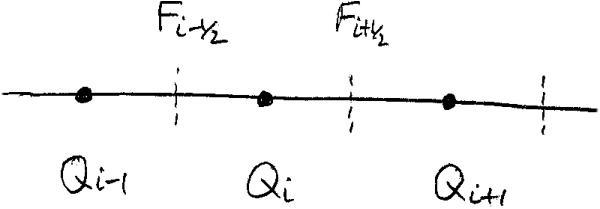
\includegraphics[width=0.4\textwidth]{figs/cellfluxsketch}

\vspace{12mm}
\item for ii) we can already do better (e.g.~RK2a from MOL)
\item for iii) we will do better (slope-limiters)
\end{itemize}
\end{frame}


\begin{frame}{a \Matlab code to play with}

\begin{itemize}
\item mostly I have been playing with PETSc, but \dots
\item upwind and Lax-Wendroff for scalar advection are implemented in this simple \Matlab code:

\begin{center}
\href{http://bueler.github.io/programs/adcompare.m}{\texttt{bueler.github.io/programs/adcompare.m}}
\end{center}
\end{itemize}
\end{frame}


\section{linear systems}

\begin{frame}{linear systems: examples}

\begin{itemize}
\item linear, constant-coefficient system for $\bq(t,x) \in \RR^d$ with $A\in\RR^{d\times d}$:
  $$\bq_t + A\, \bq_x=0$$

\setlength{\itemindent}{11mm}
\item[example:] \emph{acoustics} (and classic wave equation)
        $$\bq = \begin{bmatrix} p \\ u \end{bmatrix}, \,\, A = \begin{bmatrix} 0 & K_0 \\ \frac{1}{\rho_0} & 0 \end{bmatrix} \quad \implies \quad \begin{matrix} p_t + K_0 u_x = 0 \\ u_t + \frac{1}{\rho_0} p_x = 0 \end{matrix}$$
\item[example:] \underline{linearized} \emph{shallow water equations}
        $$\bq = \begin{bmatrix} h \\ h u \end{bmatrix}, \,\, A = \begin{bmatrix} 0 & 1 \\ -u_0^2+gh_0 & 2 u_0 \end{bmatrix} \, \implies \, {\footnotesize \begin{matrix} {\large \strut} h_t + (hu)_x = 0 \\ {\large \strut} (h u)_t + (-u_0^2+gh_0) h_x + 2u_0 (h u)_x = 0 \end{matrix} }$$
\item[example:] boringly decoupled
        $$\bq = \begin{bmatrix} u \\ v \\ w \end{bmatrix}, \,\, A = \begin{bmatrix} a & 0 & 0 \\ 0 & b & 0 \\ 0 & 0 & c \end{bmatrix} \, \implies \begin{matrix} u_t + a u_x = 0 \\ v_t + b v_x = 0 \\ w_t + c w_x = 0 \end{matrix}$$
\end{itemize}
\end{frame}


\begin{frame}{example: acoustics}

\begin{itemize}
\item $p(t,x)$ is gas pressure, $u(t,x)$ is gas velocity
\item assume pressure/velocity variations are small, and density $\rho_0$ and compressiblity $K_0$ are constant
\item thus linear, constant-coefficient first-order PDE system:
$$\begin{matrix} p_t + K_0 u_x = 0 \\ u_t + \frac{1}{\rho_0} p_x = 0 \end{matrix} \hspace{70mm}$$
\item or $\bq_t + A \bq_x=0$ where
$$\bq = \begin{bmatrix} p \\ u \end{bmatrix}, \, A = \begin{bmatrix} 0 & K_0 \\ \frac{1}{\rho_0} & 0 \end{bmatrix} \hspace{75mm}$$
\item or in 2nd-order form

with $c^2 = \frac{K_0}{\rho_0}$:
\begin{align*}
p_{tt} &= c^2 p_{xx} \hspace{70mm} \\
u_{tt} &= c^2 u_{xx}
\end{align*}
\item example solution $\longrightarrow$

\vspace{-60mm}
\hfill 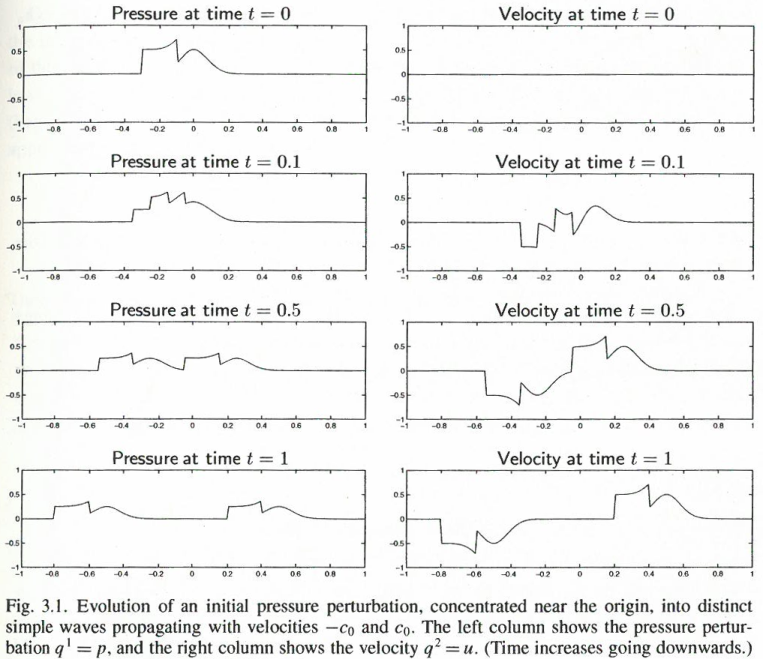
\includegraphics[width=0.55\textwidth]{figs/leveque3p1}
\end{itemize}
\end{frame}


\begin{frame}{hyperbolic systems}

\begin{definition} a first-order system $\bq_t + A\, \bq_x=0$ is \emph{hyperbolic} if $A$ is diagonalizable and all of the eigenvalues of $A$ are real
\end{definition}

\begin{itemize}
\item \emph{diagonalizable} means there is a $\RR^d$ basis of eigenvectors of $A$
\item consider \emph{left eigenvectors} of $A$, namely vectors $\bw_k \in \RR^d$ so that
    $$\bw_k^\top A = \lambda_k \bw_k^\top$$

\vspace{-2mm}
    \begin{itemize}
    \item[$\circ$] $\lambda_k$ are \emph{eigenvalues}, real numbers if the system is hyperbolic
    \item[$\circ$] $\bw_k$ are column vectors so $\bw_k^\top$ are row vectors
    \item[$\circ$] $\bw_k$ are right eigenvectors of $A^\top$: \qquad $A^\top \bw_k = \lambda_k \bw_k$
    \item[$\circ$] note that the left/right eigenvalues are the same
    \end{itemize}

\item I'll use bold for column vectors, e.g.~$\bu\in\RR^d$
    \begin{itemize}
    \item[$\circ$] note inner product: \quad $\bu^\top \bv = \ip{\bu}{\bv}$
    \end{itemize}
\end{itemize}
\end{frame}


\begin{frame}{eigenvectors decouple hyperbolic systems}

\begin{itemize}
\item assume the system $\bq_t + A\, \bq_x=0$ is hyperbolic
\item decouple it by multiplying by $\bw_k^\top$:
\begin{align*}
\bw_k^\top \bq_t + \bw_k^\top A\, \bq_x &= 0 \\
\bw_k^\top \bq_t + \lambda_k \bw_k^\top \bq_x &= 0
\end{align*}
\item define the scalar functions
    $$v_k(t,x) = \bw_k^\top \bq(t,x)$$
\item so these scalar functions satisfy decoupled advection equations:
   $$(v_k)_t + \lambda_k (v_k)_x = 0$$
\item solve these one-way advection problems by characteristics:
   $$v_k(t,x) = v_k(0,x-\lambda_k t)$$
\item matrix $A$ must be constant for this calculation
\end{itemize}
\end{frame}


\begin{frame}{eigenvectors decouple hyperbolic systems 2}

\begin{itemize}
\item the functions $v_k(t,x)$ are called \emph{Riemann invariants}:
    $$v_k(t,x) = \bw_k^\top \bq(t,x) = v_k(0,x-\lambda_k t) = \bw_k^\top \bq(0,x-\lambda_k t)$$
\item how to write the solution for $\bq(t,x)$ if we have $v_k(t,x)$?
\item we may expand in basis $\bw_k$, with scalar coefficients $c_k(t,x)$:
    $$\alert{\bq(t,x) = \sum_{k=1}^d c_k(t,x) \bw_k}$$
\item thus: \qquad $\ds \bw_\ell^\top \bq(t,x) = \sum_{k=1}^d c_k(t,x) \bw_\ell^\top \bw_k$
\item solve using (invertible) matrix $B\in \RR^{d\times d}$ with entries \alert{$B_{lk} = \bw_\ell^\top \bw_k$}:
    $$B \bc = \bv \qquad \iff \qquad \alert{\sum_{k=1}^d B_{lk} c_k(t,x) = \bw_\ell^\top \bq(0,x-\lambda_\ell t)}$$
\item \alert{red equations} combine into a solution
\item in fact we can do most examples by hand without forming $B$
\end{itemize}
\end{frame}


\begin{frame}[fragile]
\frametitle{left eigenvectors, transposes, and \Matlab}

\begin{itemize}
\item left eigenvectors for $A$ are the same as right eigenvectors for $A^\top$
\item in \Matlab, find left eigenvectors $\bw_k$ by applying \texttt{eig()} to \texttt{A'}$=A^\top$:
\begin{Verbatim}[fontsize=\small]
>> A = [...; ...; ...];     % input square matrix A
>> [X,D] = eig(A');
>> lamk = D(k,k);           % eigenvalue
>> wk = X(:,k);             % left eigenvector
\end{Verbatim}
\end{itemize}
\end{frame}


\begin{frame}{Riemann solver}

\begin{itemize}
\item in a FV scheme at some time $t_n$ we will have two different values on either side of the cell face at $x_{i+1/2}$:
    $$\bQ_{i} = \bQ_L, \quad \bQ_{i+1} = \bQ_R \hspace{50mm}$$

\vspace{-12mm}
\hfill 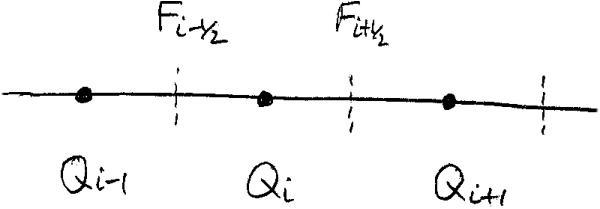
\includegraphics[width=0.4\textwidth]{figs/cellfluxsketch}

\medskip
\item $\bbf(\bq) = A\bq$ is a function of $\bq$, so to get flux $\bF_{i+1/2}$ we must know the solution on the face: $\bq(t,x_{i+1/2})$ for $t > t_n$
\item a \emph{Riemann solver} solves this problem:

\bigskip
find $\bq(t,x_{i+1/2})$, thus $\bF_{i+1/2}(t)$,

for $t > t_n$, given
\begin{align*}
\bq_t + \bbf(\bq)_x &= 0 \\
\bq(t_n,x) &= \begin{cases} \bQ_L, & x < x_{i+1/2} \\
                            \bQ_R, & x > x_{i+1/2} \end{cases} \hspace{60mm}
\end{align*}

\vspace{-30mm}
\hfill 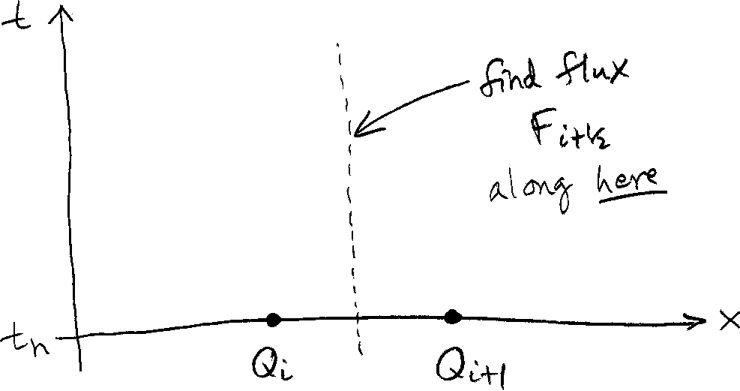
\includegraphics[width=0.44\textwidth]{figs/rsolversketch}
\end{itemize}
\end{frame}


\begin{frame}{forward versus backward characteristics}

\begin{itemize}
\item when constructing numerical schemes there are two ways of thinking about characteristics:
    \begin{itemize}
    \item[i)] Riemann solvers generate a flux at $x_*$ at times $t>t_n$
    \item[ii)] FD methods (e.g.~Lax-Wendroff) find solution at $t_{n+1}$ by going back to $t_n$
    \end{itemize}
\item 

\medskip

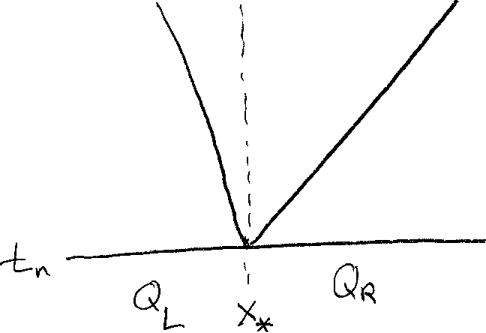
\includegraphics[height=0.34\textheight]{figs/rscharssketch} \hfill 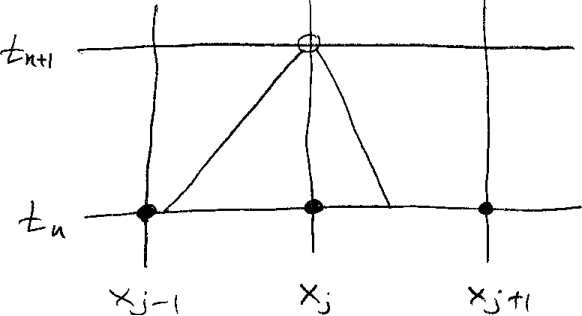
\includegraphics[height=0.38\textheight]{figs/fdcharssketch}

\medskip
\qquad Riemann solver view \hfill finite difference (FD) view \qquad \phantom{x}

\item the Riemann solver view makes it easier to
    \begin{itemize}
    \item[$\circ$] generalize to nonlinear systems
    \item[$\circ$] work with the MOL equations (w/o choosing time-stepping)
    \end{itemize}
\end{itemize}
\end{frame}


\begin{frame}{Riemann solver for the acoustics problem}

\begin{itemize}
\item recall the acoustics problem $\bq_t + A \bq_x = 0$:
        $$\bq = \begin{bmatrix} p \\ u \end{bmatrix}, \,\, A = \begin{bmatrix} 0 & K_0 \\ \frac{1}{\rho_0} & 0 \end{bmatrix} \quad \implies \quad \begin{matrix} p_t + K_0 u_x = 0 \\ u_t + \frac{1}{\rho_0} p_x = 0 \end{matrix}$$
\item eigen-decomposition of $A$:
\begin{align*}
\lambda_1 &= -c_0, \quad \bw_1 = \begin{bmatrix} 1 \\ -Z_0 \end{bmatrix} & \lambda_2 = +c_0, \quad \bw_2 = \begin{bmatrix} 1 \\ +Z_0 \end{bmatrix}
\end{align*}
where \, $c_0 = \sqrt{K_0/\rho_0}$ \, and \, $Z_0=\rho_0 c_0$
\item thus the Riemann invariants $v_k(t,x) = \bw_k^\top \bq(t,x)$ are:
\begin{align*}
v_1(t,x) &= p(t,x) - Z_0 u(t,x), & v_2(t,x) &= p(t,x) + Z_0 u(t,x)
\end{align*}
\end{itemize}
\end{frame}


\begin{frame}{Riemann solver for the acoustics problem 2}

\begin{itemize}
\item denote $x_*=x_{i+1/2}$ and let $\quad \bQ_L = \begin{bmatrix} p_L \\ u_L \end{bmatrix}, \quad \bQ_R = \begin{bmatrix} p_R \\ u_R \end{bmatrix}$
\item $\lambda_1 < 0$ so $v_1$ is left-going, so we solve forward from $t=t_n$:
\begin{align*}
p(t,x_*) - Z_0 u(t,x_*) &= v_1(t,x_*) = v_1(t_n,x_*-\lambda_1 (t-t_n)) \\
   &= p_R - Z_0 u_R
\end{align*}
\item $\lambda_2 > 0$ so $v_2$ is right-going:
\begin{align*}
p(t,x_*) + Z_0 u(t,x_*) &= v_2(t,x_*) = v_2(t_n,x_*-\lambda_2 (t-t_n)) \\
   &= p_L - Z_0 u_L
\end{align*}
\item solve for the solution at the face, namely $\bq(t,x_*)$:
\begin{align*}
\alert{p(t,x_*)} &\alert{= \frac{1}{2} \left(p_L + p_R + Z_0 (u_L - u_R)\right)} \\
\alert{u(t,x_*)} &\alert{= \frac{1}{2} \left(\frac{1}{Z_0} (p_L - p_R) + u_L + u_R)\right)}
\end{align*}
\item thus the face flux is \alert{computable} by the Riemann solver:
    $$\alert{\bF_{i+1/2}(t) =} A \bQ(t,x_*) = \alert{\begin{bmatrix} K_0 u(t,x_*) \\ \frac{1}{\rho_0} p(t,x_*) \end{bmatrix}}$$
\end{itemize}
\end{frame}


\begin{frame}{flux boundary conditions, and the grid}

\begin{itemize}
\item boundary conditions at $x=a,b$
\item easiest if think in terms of the value of the \emph{flux} there,
\item \dots thus we set up the grid to have cell faces at $x=a,b$

\medskip
\begin{center}
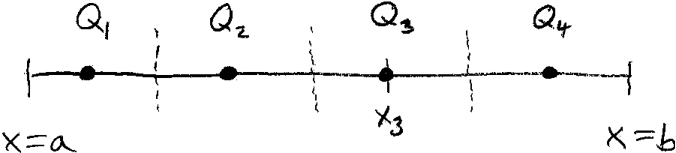
\includegraphics[width=0.45\textwidth]{figs/fluxbdrysketch}
\end{center}

\vspace{-2mm}
    $$x_j = a + (j-1/2) \Delta x \quad \text{ where } \quad \Delta x = \frac{b-a}{J}$$

\item for the acoustics problem, suppose
    \begin{itemize}
    \item[$\circ$] at $x=a$ have reflecting condition: $u(t,a)=0$
    \item[$\circ$] at $x=b$ have outflow condition: $v_1(t,b)=0$
    \end{itemize}
\item modify the Riemann solvers at $x=a$ and $x=b$ accordingly

\vspace{3mm}
\begin{center}
\alert{SHOW MOVIE}
\end{center}
\end{itemize}

% ./riemann -da_grid_x 500 -ts_max_time 5 -limiter mc -ts_monitor binary:t.dat -ts_monitor_solution binary:q.dat
% make petscPyScripts
% mkdir acoustic
% ./plotTS.py -mx 500 -dof 2 -c 0 -ylabel "p (pressure)" -ax -1.0 -bx 1.0 -cellcentered -oroot acoustic/bar t.dat q.dat
% cd acoustic/
% eog bar*.png
\end{frame}


\begin{frame}{summary of systems and Riemann solvers}

\begin{itemize}
\item if a linear system $\bq_t + A\, \bq_x=0$ in $\RR^d$ is \alert{\emph{hyperbolic}} then (by definition) it can be decoupled ($\bw_k^\top A = \lambda_k \bw_k$) into $d$ scalar (real) advection problems
\item the solutions of these advection problems, forward from time $t_n$, are the \alert{\emph{Riemann invariants}}:
    $$v_k(t,x) = \bw_k^\top \bq(t,x) = v_k(t_n,x-\lambda_k (t-t_n))$$
\item now write in conservation form: $\bq_t + \bbf(\bq)_x=0$ where $\bbf(\bq) = A\bq$
\item in the FV \alert{\emph{method-of-lines (MOL)}} view we only integrate in space:
    $$\frac{d\bQ_j}{dt} + \frac{\bF_{i+1/2} - \bF_{i-1/2}}{\Delta x} = 0$$
\item a \alert{\emph{Riemann solver}} finds the face fluxes $\bF_{i+1/2}=A \bQ^*$ by solving the \emph{Riemann problem}, with $\bQ_L,\bQ_R$ on sides of the face, to find $\bQ^*$ on the face
    \begin{itemize}
    \item[$\circ$] this uses the Riemann invariants
    \end{itemize}
\item mostly generalizable to nonlinear systems: use $A=\bbf'(\bq)$
\end{itemize}
\end{frame}


\section{high-resolution methods}

\begin{frame}{Godunov's barrier theorem}

\begin{itemize}
\item can we do better than Lax-Wendroff, even for scalar advection?
\item can we have high accuracy without oscillations? recall:
    \begin{itemize}
    \item[$\circ$] upwinding is only first-order accurate,\footnote{$O(\Delta t + \Delta x)$ local truncation error as $\Delta t\to 0$ and $\Delta x \to 0$; LW has $O(\Delta t^2 + \Delta x^2)$} but it avoids oscillations
    \item[$\circ$] Lax-Wendroff is second-order but it generates oscillations beyond the range of the initial condition
    \end{itemize}
\item rough answer: \alert{NO}

\medskip
\begin{theorem}[\emph{Godunov, 1959}]  A monotonicity-preserving \alert<2>{linear} scheme for $q_t + a q_x=0$ cannot have second-order (or higher) local truncation error in $x$.\end{theorem}

\item ``monotonicity-preserving'' means (essentially) that the scheme does not add oscillations
\item Godunov's theorem is the beginning of modern hyperbolic PDE solvers
    \begin{itemize}
    \item[$\circ$] upwinding, Lax-Friedrichs, Lax-Wendroff, leapfrog are all older
    \item[$\circ$] ``high-resolution'' schemes of the 1970--90s overcame the barrier \only<2>{\quad \alert{how?}}
    \end{itemize}
\end{itemize}
\end{frame}


\begin{frame}{the reconstruct-evolve-average view of schemes}

\begin{itemize}
\item if we want to kill oscillation then another view is helpful
\item consider: $q_t + a q_x=0$ for $a>0$, where values $\{Q_i^n\}$ are on two levels, and Euler step from $t_n$ (left) to $t_{n+1}$ (right) w.~1st-order upwinding:

\begin{center}
\quad 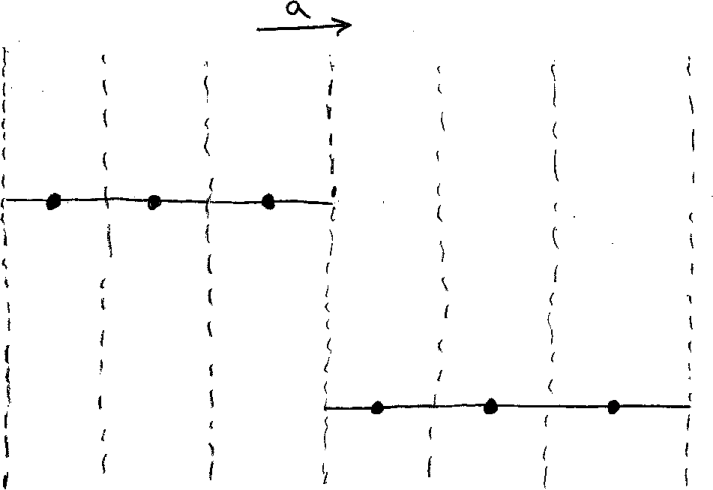
\includegraphics[width=0.3\textwidth]{figs/upreconstructleft} \qquad 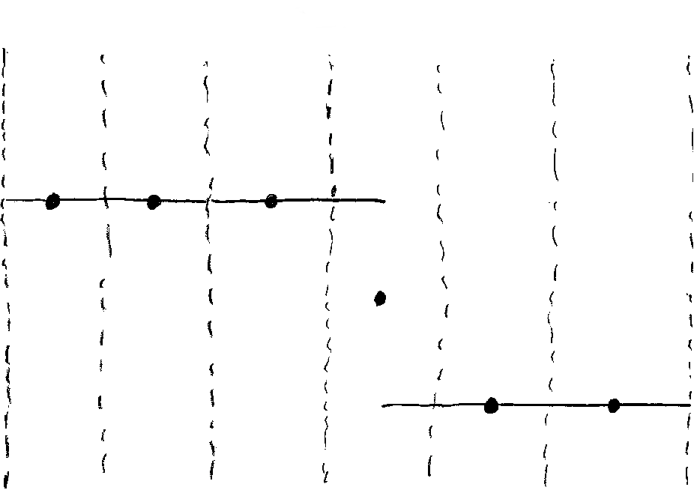
\includegraphics[width=0.3\textwidth]{figs/upreconstructright}
\end{center}

    \begin{itemize}
    \item[$\circ$] upwinding uses constant values (zero slope) in cells
    \item[$\circ$] dots on right show new cell averages
    \end{itemize}
\item versus Lax-Wendroff, which uses downwind slope:

\begin{center}
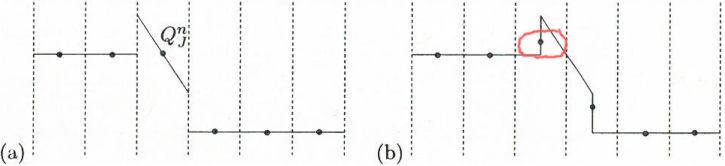
\includegraphics[width=0.69\textwidth]{figs/leveque6p4}
\end{center}

    \begin{itemize}
    \item[$\circ$] note the \alert{overshoot}, which we want to avoid
    \end{itemize}
\end{itemize}
\end{frame}


\begin{frame}{slope reconstruction}

\begin{itemize}
\item at time $t_n$ we only know the discrete unknowns $\{Q_j^n\}$
\item but we can attempt to ``reconstruct'' a linear function $\tilde q(t_n,x)$ on each cell $x_{i-1/2} \le x \le x_{i+1/2}$:
    $$\tilde q(t_n,x) = Q_i^n + \sigma_i^n (x - x_i)$$

    \begin{itemize}
    \item[$\circ$] $\sigma_i^n$ is the \emph{slope} in the cell
    \item[$\circ$] the average remains as $Q_i^n$
    \end{itemize}
\item possibilities for slope ($a>0$):
\begin{align*}
&\text{zero:}     & \sigma_i &= 0 \hspace{75mm} \\
&\text{{\color{red} downwind:}} & \sigma_i &= \frac{Q_{i+1}-Q_i}{\Delta x} \\
&\text{{\color{ForestGreen} upwind:}}   & \sigma_i &= \frac{Q_i-Q_{i-1}}{\Delta x} \\
&\text{{\color{blue} centered:}} & \sigma_i &= \frac{Q_{i+1}-Q_{i-1}}{2\Delta x}
\end{align*}

\vspace{-45mm}
\hfill 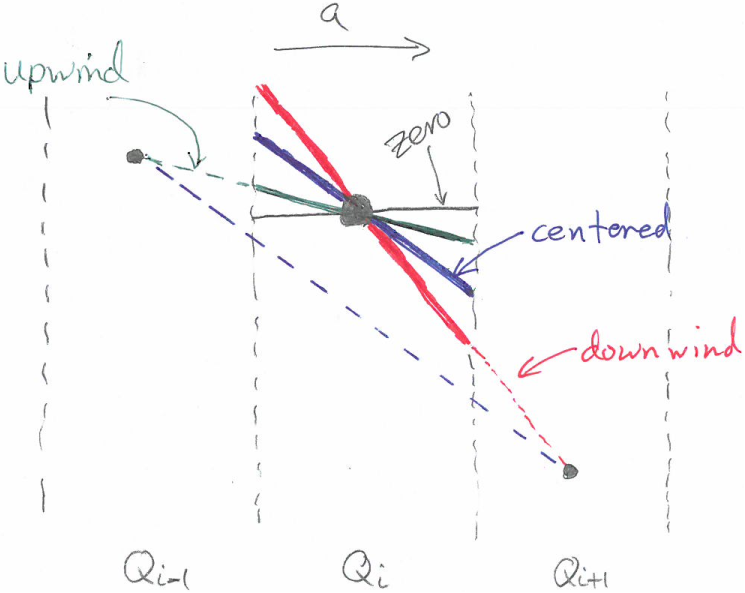
\includegraphics[width=0.47\textwidth]{figs/slopessketch}
\end{itemize}
\end{frame}


\begin{frame}{slope limiter idea}

\begin{itemize}
\item the slope limiter idea is to use one of these slopes to get higher accuracy \emph{except} if using that slope puts the reconstruction out of range of the values $\{Q_{i-1},Q_i,Q_{i+1}\}$
\item \alert{$\minmod$ \emph{slope limiter}:}
    $$\sigma_i = \minmod\left\{\frac{Q_i-Q_{i-1}}{\Delta x},\frac{Q_{i+1}-Q_i}{\Delta x}\right\}$$

    \begin{itemize}
    \item[$\circ$] by definition, for real numbers $a,b$ of the same sign:
        $$\minmod\{a,b\} = \begin{cases} 0, & ab \le 0 \\
                                         a, & ab>0 \text{ and } |a| \le |b| \\
                                         b, & ab>0 \text{ and } |a| > |b| \end{cases}$$
    \item[$\circ$] in words: $\minmod\{a,b\}$ is closest of $a$ or $b$ to zero unless they differ in sign; then it is zero
    \end{itemize}
\end{itemize}
\end{frame}


\begin{frame}{slope limiter idea 2}

\begin{itemize}
\item another, recommended, alternative is the \alert{\emph{MC slope limiter}:}
    $$\sigma_i = \minmod\left\{\frac{Q_{i+1}-Q_{i-1}}{2\Delta x},2\minmod\Big\{\frac{Q_i-Q_{i-1}}{\Delta x},\frac{Q_{i+1}-Q_i}{\Delta x}\Big\}\right\}$$
\item in pictures:

\begin{center}
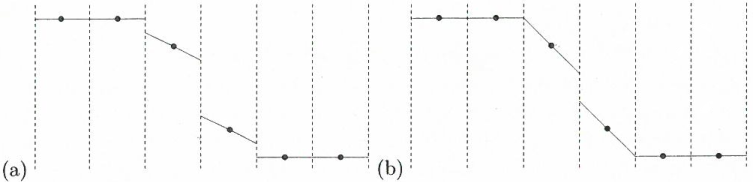
\includegraphics[width=0.9\textwidth]{figs/leveque6p5}
\end{center}

\hspace{15mm} $\minmod$ limiter \hfill MC limiter \hspace{15mm} \phantom{x}
\item can you draw-in the downwind (i.e.~Lax-Wendroff) case in your head?  it has overshoots
\item theory of \emph{total variation diminishing} (TVD) schemes, circa 1990s, arises from these pictures
\end{itemize}
\end{frame}


\begin{frame}{results for advection equation}

\begin{itemize}
\item consider scalar advection again: $q_t + a q_x=0$, $a=1$, periodic b.c.s
\end{itemize}

\begin{center}
\includegraphics<1>[width=0.7\textwidth]{figs/leveque6p1} \includegraphics<2>[width=0.7\textwidth]{figs/leveque6p2}
\end{center}
\end{frame}


\begin{frame}{MOL slope limiting and Riemann solvers}

\begin{itemize}
\item one detail \dots
\item suppose we want to use limited slopes \emph{and} build Riemann solvers, \emph{in the method-of-lines (MOL) framework}
\item then we first apply the slope-limiter as usual, \dots
\item and then compute the flux $\bF_{i-1/2}$ in terms of this picture:

\medskip
\begin{center}
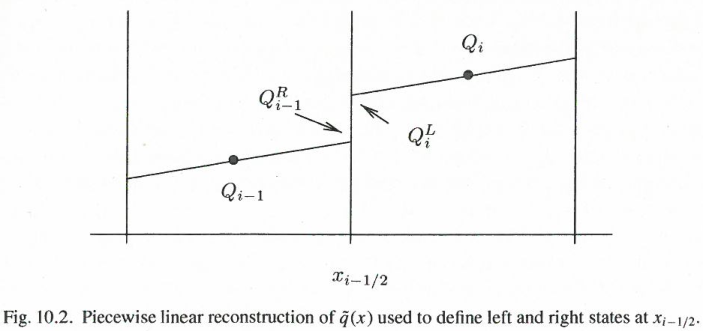
\includegraphics[width=0.6\textwidth]{figs/leveque10p2}
\end{center}
\item the left and right values at the face, $\bQ_{i-1}^R$ and $\bQ_i^L$, are the ones seen by (used in) the Riemann solver to compute the solution value at the face forward in time, and thus the flux $\bF_{i-1/2}(t)$ for $t>t_n$
\end{itemize}
\end{frame}


\section{nonlinear conservation laws}

\begin{frame}{conservation laws}

\begin{itemize}
\item a \emph{conservation law} is a first-order system for $\bq(t,x) \in \RR^d$ with a given \emph{flux function} $\bbf:\RR^d\to \RR^d$:
  $$\bq_t + \bbf(\bq)_x=0$$
    \begin{itemize}
    \item[$\circ$] $\bbf$ could depend on $t$ or $x$: \qquad $\bq_t + \bbf(t,x,\bq)_x=0$
    \item[$\circ$] there could be a right-hand side: \qquad $\bq_t + \bbf(t,x,\bq)_x=\bg(t,x,\bq)$
    \item[$\circ$] the conservation law is linear if $\bbf(\bq) = A\bq$
    \item[$\circ$] if $\bbf$ depends on $\grad \bq$ \dots e.g.~heat equation \dots then the system is not hyperbolic
    \end{itemize}

\bigskip
\item two scalar, nonlinear examples:
    \begin{itemize}
    \item[$\circ$] \emph{Burger's equation} with $f(q)=\frac{1}{2} q^2$:
        $$q_t + \left(\tfrac{1}{2} q^2\right)_x = 0 \qquad \iff \qquad q_t + q q_x = 0$$
    \item[$\circ$] \emph{nonlinear traffic model} with $f(q)=u_{\max} (1-q) q$:
        $$q_t + \left(u_{\max} (1-q) q\right)_x = 0$$
    \end{itemize}
\end{itemize}
\end{frame}


\begin{frame}{nonlinear conservation laws: system examples}

\begin{itemize}
\setlength{\itemindent}{11mm}
\item[example:] \emph{shallow water equations} with height $h(t,x)$ and velocity $u(t,x)$:
        $$\bq = \begin{bmatrix} h \\ hu \end{bmatrix}, \, \bF(\bq) = \begin{bmatrix} h \\ h u^2 + \frac{g}{2} h^2 \end{bmatrix} \quad \implies \quad \begin{matrix} h_t + (hu)_x = 0 \\ (hu)_t + \Big(h u^2 + \frac{g}{2} h^2\Big)_x = 0 \end{matrix}$$
\item[example:] \emph{Euler equations for an ideal gas}:
        $$\bq = \begin{bmatrix} \rho \\ \rho u \\ E \end{bmatrix}, \, \bF(\bq) = \begin{bmatrix} \rho u \\ \rho u^2 + p \\ (E+p) u \end{bmatrix} \quad \implies \quad \begin{matrix} \rho_t + (\rho u)_x = 0 \\ (\rho u)_t + \Big(\rho u^2 + p\Big)_x = 0 \\ E_t + \Big((E+p) u\Big)_x = 0 \end{matrix}$$
    \begin{itemize}
    \item[$\circ$] variables are density $\rho(t,x)$, velocity $u(t,x)$, and energy density $E(t,x)$
    \item[$\circ$] the pressure $p$ is found from an equation of state, for example for a polytropic ideal gas ($\gamma \approx 1.4$ for air):
        $$E = \frac{p}{\gamma - 1} + \frac{1}{2} \rho u^2$$
    \end{itemize}
\end{itemize}
\end{frame}


\begin{frame}{traffic model}

\begin{itemize}
\item let us consider a scalar conservation law first
\item $q(t,x)$ is the density of cars, $0\le q \le 1$
\item they move at speed
    $$U(q) = u_{\max} (1-q)$$

    \begin{itemize}
    \item[$\circ$] they slow down when the density is high
    \end{itemize}
\item as conservation law $q_t + f(q)_x = 0$, the flux of cars is
    $$f(q) = U(q) q = u_{\max} (1-q) q$$
\item note that
    $$f'(q) = u_{\max} (1-2q)$$
\item thus nonlinear equation is like scalar advection:
    $$q_t + f'(q) q_x = 0$$

    \begin{itemize}
    \item[$\circ$] characteristic speed is $a = f'(q) = u_{\max} (1-2q)$
    \end{itemize}
\end{itemize}
\end{frame}


\begin{frame}{traffic: speed versus speed}

\begin{itemize}
\item speed of car is $U(q) = u_{\max} (1-q)$
\item speed of characteristic is $f'(q) = u_{\max} (1-2q)$
\end{itemize}

\begin{center}
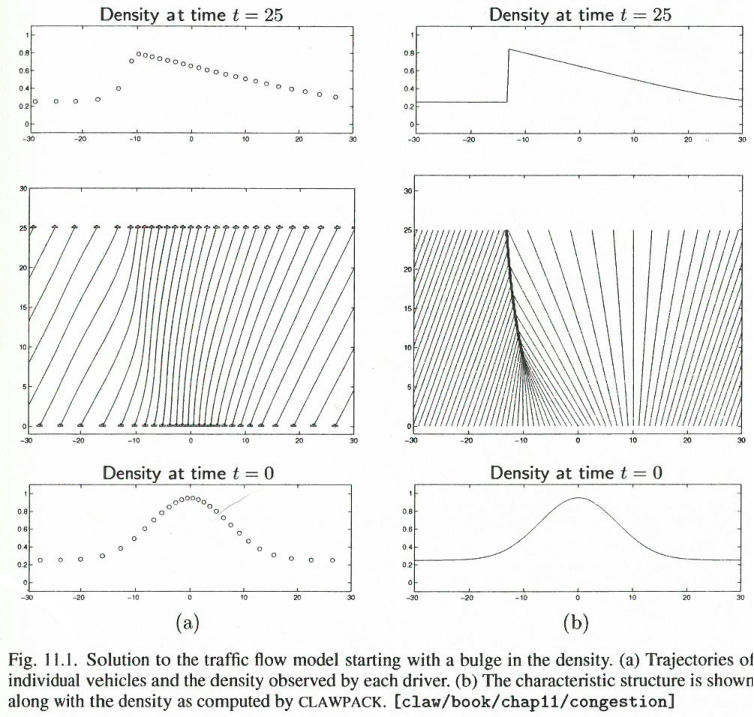
\includegraphics[width=0.68\textwidth]{figs/leveque11p1}
\end{center}
\end{frame}


\begin{frame}{traffic: shock and rarefaction waves}

\begin{itemize}
\item previous slide shows formation of a \emph{shock wave} from a smooth hump
\item the model can also form \emph{rarefaction waves}
\end{itemize}

\begin{center}
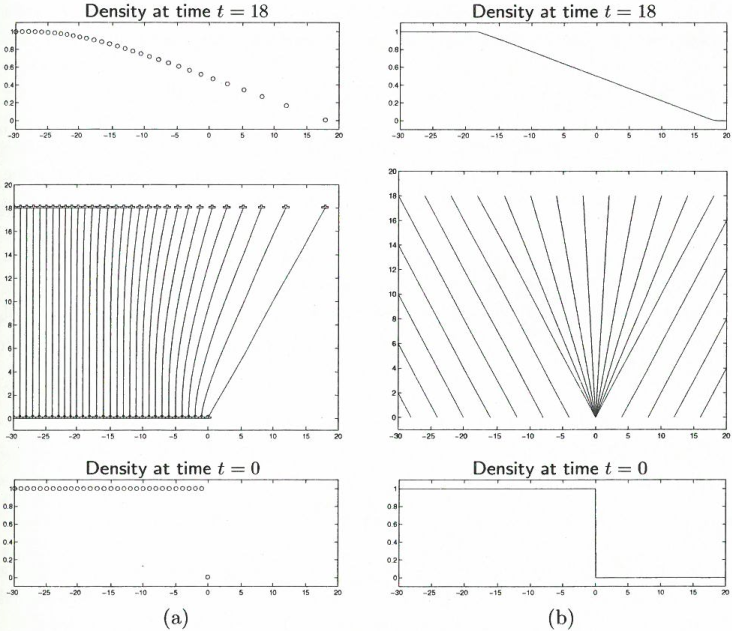
\includegraphics[width=0.65\textwidth]{figs/leveque11p3}
\end{center}
\end{frame}


\begin{frame}{Riemann solver for traffic equation}

\begin{itemize}
\item $F(q) = U(q) q$ and $U(q) = u_{\max} (1-q)$
\end{itemize}

\hfill 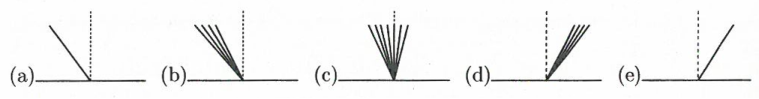
\includegraphics[width=0.75\textwidth]{figs/leveque12p1}
\end{frame}


\begin{frame}{shallow water equations}

\begin{itemize}
\item $h(t,x)$ is height above equilibrium, $u(t,x)$ is horizontal water velocity
\item FIXME
\end{itemize}
\end{frame}


\begin{frame}{shallow water: illustration}

\begin{itemize}
\item dam break example

\hfill 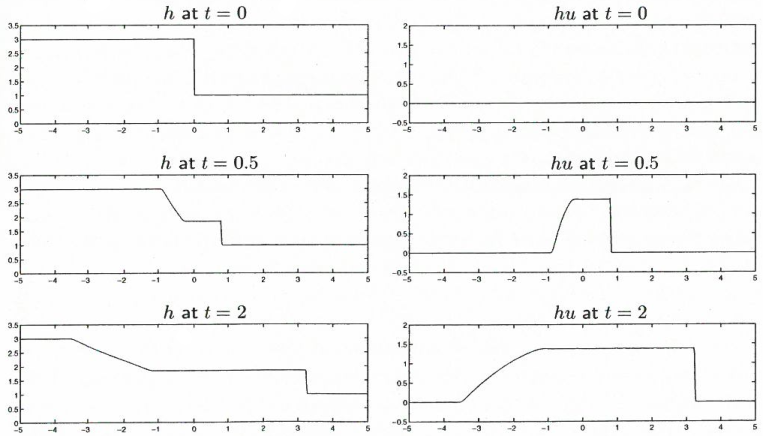
\includegraphics[width=0.75\textwidth]{figs/leveque13p4}

\end{itemize}
\end{frame}


\begin{frame}{shallow water: my results}

\begin{itemize}
\item FIXME with \texttt{riemann.c}
\end{itemize}

\vspace{10mm}
\begin{center}
\alert{SHOW MOVIE}
\end{center}
\end{frame}


\begin{frame}{summary}

\begin{itemize}
\item for hyperbolic conservation-law systems
    \begin{itemize}
    \item[$\circ$] linear: acoustics, elasticity, Maxwell's equations
    \item[$\circ$] nonlinear: shallow water, compressible gas equations
    \end{itemize}
a preferred numerical approach since the 1990s is a
\begin{center}
\alert{high-resolution Godunov method}
\end{center}
\item consists of three things:
    \begin{itemize}
    \item[\alert{1.}] \alert{finite volume thinking}
        \begin{itemize}
        \item conservation law is spatially integrated
        \item discrete unknowns are cell averages
        \item flux is needed at faces between cells
        \end{itemize}
    \item[\alert{2.}] \alert{Riemann solvers}
        \begin{itemize}
        \item a ``Riemann problem'' considers different cell values on each side of a face
        \item a Riemann solver determines the local wave structure (rarefaction, shock)
            \begin{description}[abc]
            \item[$\diamond$] computes the flux on the face
            \item[$\diamond$] provided by the user
            \item[$\diamond$] exact or approximate (e.g.~Roe for shallow water)
            \end{description}
        \end{itemize}
    \item[\alert{3.}] \alert{slope limiters}
        \begin{itemize}
        \item first-order upwinding: solution is constant in a cell (``classical Godunov'')
        \item for higher-order without oscillations:
            \begin{description}[abc]
            \item[$\diamond$] solution is ``reconstructed'' with slope in each cell
            \item[$\diamond$] slope is (nonlinearly) limited
            \end{description}
        \end{itemize}
    \end{itemize}
\end{itemize}
\end{frame}


\section{scalar advection in 2D}

\begin{frame}{finite volumes in 2D}

\begin{itemize}
\item equation $q_t + \Div \bF(q) = 0$
\item for example, $\bF(q) = \ba q$ where $\ba(x,y) = \left<u(x,y), v(x,y)\right>$ is a velocity field
\item that is,
    $$q_t + (u q)_x + (v q)_y = 0$$
\end{itemize}

\hfill 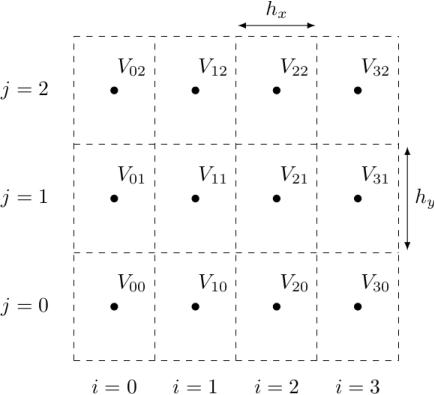
\includegraphics[width=0.4\textwidth]{figs/bueler11p1}
\end{frame}


\begin{frame}{flux-limiter higher-resolution schemes}

\begin{itemize}
\item x
\end{itemize}
\end{frame}


\begin{frame}{implementation of flux-limiter in 2D}

\begin{itemize}
\item x
\item see \texttt{c/ch11/advect.c} at \href{https://github.com/bueler/p4pdes}{\texttt{github.com/bueler/p4pdes}}
\end{itemize}

\begin{center}
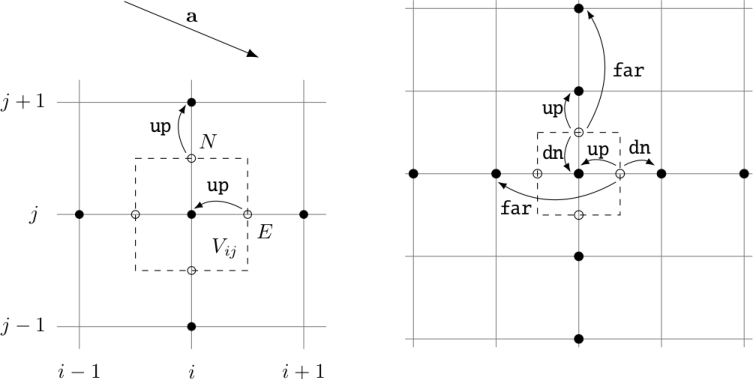
\includegraphics[width=0.6\textwidth]{figs/bueler11p8}
\end{center}

\end{frame}


\begin{frame}{results}

\begin{itemize}
\item x
\end{itemize}

\hfill 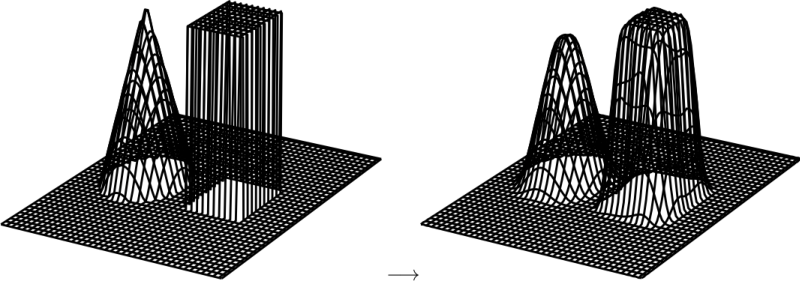
\includegraphics[width=0.75\textwidth]{figs/bueler11p7}
\end{frame}


\begin{frame}{movie}

\begin{itemize}
\item domain is square $\Omega = (-1,1) \times (-1,1)$
\item $q_t + \Div \bF(q) = 0$ where $\bF(q) = \ba q$ and $\ba$ is pure rotation:
    $$\ba(x,y) = \left<y,-x\right>$$
\item again, see \texttt{c/ch11/advect.c} at \href{https://github.com/bueler/p4pdes}{\texttt{github.com/bueler/p4pdes}}
\end{itemize}

\vspace{10mm}
\begin{center}
\alert{SHOW MOVIE}
\end{center}

% cd p4pdes/c/ch11
% make advect
% ./advect -da_refine 4 -adv_problem rotation -ts_max_time 6.283 -ts_monitor_solution draw
\end{frame}

\end{document}

